\chapter{Testing}

In questo capitolo veranno descritte le metodologie di test.

\section{Testing della servlet}
Sono stati definiti alcuni test per verificare il funzionamento delle principali parti del programma.
Alcuni sono stati realizzati tramite la libreria \textit{JUnit} di Java, mentre altri sono stati eseguiti manualmente.

\subsection{Parsing dei parametri}
In questo unit test viene verificata la correttezza della funzione \textit{parseCommandLineParameters}, che esegue il parsing dei parametri specificati tramite linea di comando.
Essendo i parametri scritti dall'utente, è ragionevole pensare che possano essere commessi errori nella digitazione.
Di conseguenza, si è ritenuto utile implementare e verificare il corretto funzionamento di una funzione di questo tipo.

\subsection{Parsing dei messaggi JSON in input}
In questo test viene generata una richiesta HTTP alla servlet, sul modello di quelle provenienti dai Raspberry. Il test verifica che tale richiesta contenga dati JSON sintatticamente e semanticamente corretti.

\subsection{Scrittura di un record sul database}
In questo test viene verificata la corretta comunicazione tra servlet e database, inviando al database una richiesta REST che comporta la scrittura di un record.
Il database invierà l'esito dell'operazione nella risposta. In base al successo o al fallimento dell'operazione, verrà restituito un messaggio di stato HTTP descrittivo.

\subsection{Test di carico}
Poiché i Raspberry sono collegati ad un'istanza della servlet con un rapporto di cardinalità molti a uno, è necessario che la servlet sia in grado di gestire correttamente più richieste contemporaneamente.
In base a quanto affermato in fase di analisi dei requisiti, il caso pessimo è rappresentato da un centinaio o poco più di richieste concorrenti.
Sebbene tale caso pessimo sia molto distante da quello medio, si è valutato di verificare il comportamento della servlet con un carico di quelle dimensioni.
\\Dai test effettuati, emerge che con l'aumentare delle richieste contemporanee, aumenta il tempo necessario ad elaborarle tutte.
Tuttavia, su una rete a bassa latenza, anche con 150 richieste contemporanee la servlet non mostra particolari difficoltà, in quanto tutte vengono elaborate prima che vadano in timeout.
Si ritiene che con un tale volume di richieste non si riscontrino particolari problemi anche su reti a media latenza, ma le prestazioni potrebbero essere differenti.
Poiché il tempo necessario per processare una singola richiesta è estremamente ridotto, in realtà la latenza di rete non solo non è particolarmente dannosa, ma in alcuni casi potrebbe anche contribuire ad un bilanciamento del carico nel tempo, smorzando i picchi.
In ogni caso, come precedentemente affermato, si raccomanda di non confidare eccessivamente in una singola istanza della servlet per sistemi di grandi dimensioni, ma di suddividere il carico tra più servlet.


\section{Testing della parte embedded}
Per quanto riguarda gli unit tests della parte Raspberry, si è cercato di ottenere una buona copertura delle funzioni più complesse.
In tutti i test è stato utilizzato il framework \textit{unittest} di Python, inizialmente ispirato a \textit{JUnit} di Java.

\subsubsection{Main Sanity Check \label{msc}}
In questo test si è controllata la correttezza della funzione \textit{sanity\_check} presente nel \textit{main}, richiamata durante la normale esecuzione del programma quando le policy di un lampione vengono modificate, per assicurare che i dati inseriti siano validi.
I controlli che esegue passano dai più intuitivi, come il fatto che l'orario debba essere nell'intervallo numerico 0-23, ai più complessi, come la verifica che la fascia oraria di risparmio energetico sia compresa tra l'inizio e la fine delle policy di accensione e spegnimento.
\\Poiché l'inserimento di fasce orarie include alcuni casi particolari come l'inizio delle policy in un giorno e la fine nel seguente, scrivere un test per validare l'input è di notevole aiuto per prevenire molti errori che potrebbero presentarsi nell'utilizzo reale.
In questo caso, potendo essere influente anche il giorno e l'orario in cui si effettua il controllo, si è utilizzata la funzione \textit{patch} offerta da \textit{unittest.mock} per modificare a piacimento il valore relativo alla data corrente.

\subsubsection{Classe ``Lamp''}
Sulla classe \textit{lamp} sono stati testati i due metodi statici \textit{get\_delta} e \textit{get\_wait}.
\\Il metodo \textit{get\_delta} prende come parametri un orario di inizio e uno di fine, e restituisce i secondi di differenza tra i due orari.
Per questo tipo di test si è inserito un orario di inizio uguale alla fine, un orario di fine maggiore di quello di partenza, quindi relativo allo stesso giorno, e un orario di fine minore, quindi relativo al giorno seguente.
\\Il metodo \textit{get\_wait}, in modo simile a \textit{get\_delta}, prende come parametri un orario di inizio e uno di fine, e restituisce i secondi di attesa necessari all'inizio del periodo di scheduling.
Se l'orario attuale è già all'interno del periodo di scheduling, verrà restituito un valore negativo corrispondente al numero di secondi già trascorsi dall'inizio.
In questo caso sono stati effettuati diversi test combinando i possibili orari di inizio, fine e l'orario in cui viene effettuata la richiesta.
Per modificare l'orario della richiesta è stata usata la funzione \textit{patch} come nel caso precedente (sezione \ref{msc}).

\subsubsection{Classe ``RPiMockGPIO''}
Per simulare i pin di GPIO del Raspberry Pi è stata creata la classe \textit{RPiMockGPIO} in modo da simulare l'esecuzione del programma anche senza l'utilizzo fisico di un Raspberry.
Questo si rivela particolarmente utile in fase di design, quando si vuole testare il codice senza avere a disposizione l'hardware.
\\La funzione di GPIO maggiormente significativa che viene utilizzata nel programma è \textit{wait\_for\_edge} e consiste nell'attesa che un determinato pin cambi stato.
Nel progetto viene utilizzata tutte le volte che si vuole misurare la distanza con il sensore ad ultrasuoni.
Tenendo conto del tempo trascorso tra l'inizio e la fine dell'esecuzione di \textit{wait\_for\_edge} è possibile calcolare la distanza dell'oggetto in prossimità del sensore.
\\L'implementazione di \textit{wait\_for\_edge} nella classe RPiMockGPIO prevede semplicemente un \textit{time.sleep} su una variabile \textit{wait\_seconds}.
Per questo motivo, regolando il valore di \textit{wait\_seconds} è possibile simulare diversi scenari: impostando un valore alto (come ad esempio un secondo) si può simulare una situazione in cui non ci siano mezzi in transito sulle carreggiate;
impostando un valore basso (come 0.001 secondi) si potrà rilevare sempre le auto in transito.

\subsubsection{Schedule test \label{st}}
Questo test permette di controllare la correttezza durante le operazioni di inizializzazione del sistema, di accensione dei lampioni quando si è nella fascia di scheduling, e di successivo spegnimento.
\\La configurazione del test prevede:
\begin{itemize}
	\item la lettura del file di configurazione di un lampione;
	\item l'impostazione tramite mock object dell'orario corrente a dieci secondi prima dell'inizio dello scheduling;
	\item l'impostazione ad un secondo della variabile \textit{wait\_seconds}, quindi corrispondente a nessuna auto in transito.
\end{itemize}
In seguito viene eseguito il \textit{main} del programma e dopo pochi secondi si controlla che il lampione che si sta testando sia spento, in quanto fuori dal suo orario di scheduling.
Avendo impostato inizialmente l'orario corrente a dieci secondi dall'inizio dello scheduling, il sistema attende qualche secondo e poi controlla che il lampione sia acceso, come da programmazione.
La sua intensità deve corrispondere a quella impostata sul file \textit{cfg}.
Infine, si imposta l'ora corrente ad un minuto dopo la fine dello scheduling e si verifica il corretto spegnimento del lampione.

\subsubsection{Test rilevamento auto}
In questo test viene controllata la correttezza delle operazioni di inizializzazione del sistema, rilevamento di mezzi in transito sulla carreggiata, ritorno a luminosità ridotta quando non sono presenti auto e infine spegnimento alla fine dello scheduling.
\\La configurazione del test prevede:
\begin{itemize}
	\item la lettura del file di configurazione di un lampione;
	\item l'impostazione tramite mock object dell'orario corrente all'interno della fascia di scheduling di risparmio energetico;
	\item l'impostazione a zero secondi della variabile \textit{wait\_seconds}, permettendo di rilevare sempre mezzi in transito sulla carreggiata.
\end{itemize}
In seguito viene eseguito il \textit{main} e dopo pochi secondi si verifica che il lampione sia acceso, in quanto il sistema deve avere rilevato automobili sulla carreggiata.
Successivamente si imposta la variabile \textit{wait\_seconds} ad un secondo, quindi in modo che non vengano più rilevate auto.
Dopo qualche secondo di attesa si controlla che l'intensità del lampione corrisponda al suo valore di risparmio energetico.
Infine, analogamente a quanto avviene per il test precedente (sezione \ref{st}), viene impostata l'ora corrente ad un minuto dopo la fine dello schedule e si verifica che il lampione si sia spento correttamente.


\section{Prototipo}
È stato realizzato un modellino in scala (figura \ref{model}) per simulare il funzionamento del sistema: ad un Raspberry Pi sono stati collegati quattro led con l'obiettivo di rappresentare i lampioni stradali, un sensore di prossimità (per testare il rilevamento di auto) e una fotoresistenza (per testare la regolazione dei lampioni in base alla luminosità ambientale).
\begin{figure}[tbp]
	\centering
	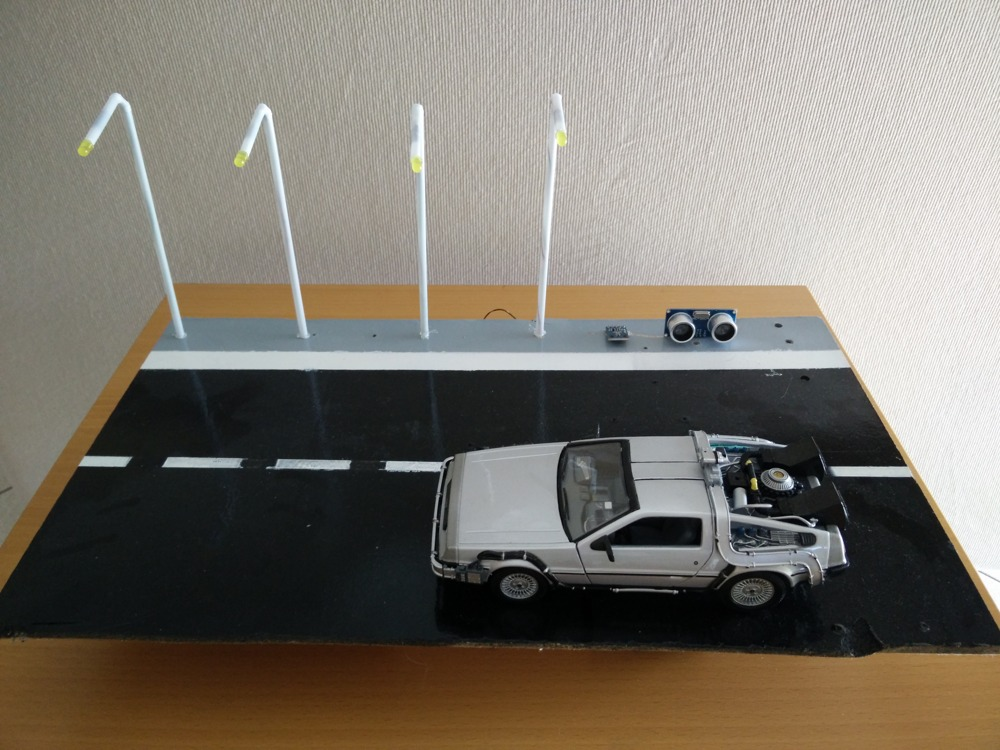
\includegraphics[width=13cm]{figure/Model.jpg}
	\caption{Modello in scala del progetto \label{model}}
\end{figure}
